  \begin{figure*}
        \centering
        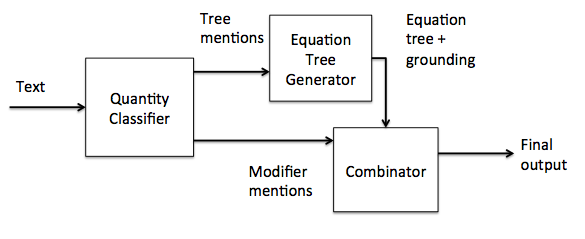
\includegraphics[height=5cm]{pipeline.png}
        \caption{Pipeline of our system}
        \label{pipeline}
  \end{figure*}


  We now describe the algorithm for identifying the terms and
  expressions of the equation from a sentence, and how we can
  construct a complete equation using them. We use the following two
  modules in a pipeline:
  \begin{enumerate}
    \item \textbf{Quantity Classifier} : This module looks at a quantity
      and decides whether it is relevant to the equation formed from
      the sentence. Also, it determines whether the
      quantity acts as a modifier in a sentence, and how it 
      modifies the corresponding variables.
      
    \item \textbf{Equation Tree Generator} : This module jointly
      grounds variables and generates an equation tree.
  \end{enumerate}

  We discuss the details of these modules in the following subsections.
  
  \subsection{Quantities Extraction and Normalization}
    The natural first step towards identifying the terms participating
    in the equation is to find the quantities mentioned in the
    sentence. We use the Illinois Quantifier package \cite{RoyViRo15}
    to detect all the quantity mentions.  The quantifier extracts
    mention spans from the text, where each span identifies a
    quantity. Each such span is represented as a triple $(v,u,c)$
    where $v$ denotes the value, $u$ denotes the unit and $c$ denotes
    the change in the quantity (if any).

    The quantity mentions identified fall into one of the following
    three categories:
    \begin{enumerate}
    \item {\bf Tree Mention} - Mentions that are part of the final
      equation tree. In Fig \ref{fig:eqparse}, ``5'' is a tree
      mention.

    \item {\bf Spurious Mentions} - Quantities which are not
      used in the equation.  In Fig \ref{fig:eqparse}, the quantity
      ``two numbers'' is a spurious mention, as the magnitude $2$
      plays no role in the final equation. This means that the
      quantity triggers arising from this mention will not be part of
      the equation tree.  Variable triggers generated using the same
      span can still be relevant to the equation tree.

    \item {\bf Modifier Mentions} - Quantities which play the
      role of modifiers. In Fig \ref{fig:eqparse}, ``10'' is a
      modifier mention, as it modifies both the variables in the
      resulting equation.
    \end{enumerate}

  \subsection{Quantity Classifier}
    We use a multiclass classifier trained on a small number of
    examples from our annotated data set, to determine the quantity
    type. Moreover, for the case of modifier mentions, there is a need
    to determine also how the modifier changes the variables in the
    problem. Since the number of outcomes is small, we predict these
    properties jointly with the quantity type. Specifically, we
    perform a multicalss classification to classify each quantity to
    one of Tree mention, Spurious mention, or a modifier conjoined
    with a modification manner.

    The features used for this module are as follows : 
    \begin{enumerate}
      \item \textbf{Lexical features} : Unigrams and bigrams generated
        from a window around the quantity.
      \item \textbf{POS Tags} : Part of speech of tags of neighborhood 
        tokens, conjoined with lexical features.
      \item \textbf{Quantity Features} : Units of the quantity, whether
        number associated with quantity is one or two.
    \end{enumerate}  
    
  \subsection{Equation Tree Generator}

    This module receives the Tree mentions detected by the Quantity
    classifier, and predicts an equation tree along with grounding of
    the variables. We formulate this problem as a structured
    prediction task.  The input structure $x$ consists of the sentence
    $S$, as well as the tree mentions detected by the Quantity
    classifier. As we pointed out earlier grounding of variables might
    be ambiguous, since multiple groundings might be valid for any
    given variable. Therefore, we model the grounding of variables as
    a latent variable $h$, and our system gets to decide which of the
    valid groundings it will use. The output structure $y$ now
    comprises of an equation tree, whose leaves are formed by the
    union of the tree mentions in $x$, and the grounded variable
    mentions $h$.

    We learn a scoring function to decide, given $x$, the best
    equation tree $y^*$ and the best grounding of variables $h^*$. We
    assume that our scoring function is of the following form :
    \begin{align*}
      f_w(y, h) &= w^T\phi(x, y, h) \\ 
    \end{align*}  
    where $\phi(x, y, h)$ is a feature vector extracted from $x, h,
    y$. The prediction $(y^*, h^*)$ is then chosen as follows:
    \begin{align*}
      (y^*, h^*) &= \arg\max_{(y, h)\in \mathcal{H} \times \mathcal{Y}} f_w(y, h)
    \end{align*}
    where $\mathcal{H}$ represents the set of all possible groundings
    of the variables, and $\mathcal{Y}$ represents the set of all
    possible equation trees.

    \subsubsection{Learning}
    \label{sec:prediction}
      We assume access to $N$ training examples of the form : $(x_1,
      H_1, y_1), (x_2, H_2, y_2), \ldots, (x_N, H_N, y_N)$, where each
      $H_i$ is a set of valid groundings possible for the variables in
      the equation tree $y_i$. This is different from most latent
      variable structured learning problems in that the domain of the
      hidden variable is explicitly constrained by $H_i$. We use a
      modified latent structural SVM to learn the weight vector
      $w$. The details of the algorithm are in Algorithm \ref{lssvm}.

      \begin{algorithm}
       \caption{Constrained Latent Structural SVM}
       \label{lssvm}
       \begin{algorithmic}[1]
         \REQUIRE Training data $T = \{(x_1, H_1, y_1), (x_2, H_2, y_2),
         \ldots, (x_N, H_N, y_N)\}$ 
         \ENSURE Trained weight vector $w$
         \STATE $w \leftarrow w_0$
         \REPEAT 
           \STATE $T' \leftarrow \emptyset$
           \FORALL {$(x_i, y_i, H_i) \in T$}
             \STATE $h_i^* \leftarrow \arg\max_{h \in H_i} w^T\phi(x_i, y_i, h)$
             \STATE $T' \leftarrow T \cup \{x_i, (y_i, h_i^*)\}$  
           \ENDFOR
           \STATE Update $w$ by running standard Structural SVM algorithm
           on $T'$
         \UNTIL{convergence}
         \RETURN $w$
       \end{algorithmic}
      \end{algorithm}


%      \begin{multline}
%        \min_w \left[ \frac{1}{2}||w||^2
%          + C\sum_{i=1}^N \max_{(\hat{y}, \hat{h})\in Y \times H}
%          \left[w\cdot \phi(x_i, \hat{y}, \hat{h}) 
%            + \Delta(y_i, \hat{y}, \hat{h}) \right] \right] \\
%        - \left[ C\sum_{i=1}^N \max_{h \in H_i} 
%          w \cdot \phi(x_i, y_i, h) \right]
%      \end{multline}
      
%      where $\Delta(y_i, \hat{y}, \hat{h})$ is a structured loss
%      suffered when, instead of gold structure $y_i$, the system
%      predicts equation tree $\hat{y}$, along with grounding
%      $\hat{h}$. 

      The distinction from standard latent structural SVM is in the
      latent variable completion problem, stated in line $5$ of Algorithm
      \ref{lssvm}. In order to get the best latent variable assignment
      $h_i^*$ for input tuple $(x_i, y_i, H_i)$, we search only inside
      $H_i$, instead of all of $\mathcal{H}$. A similar
      formulation can be found in
      \cite{ZettlemoyerCo07,BjorkelundKu14}, but in both the cases,
      the set $H_i$ can be computed deterministically from $y_i$. In
      our case, we depend on explicit annotations for $H_i$.

    \subsubsection{Inference}
      We need to solve two inference algorithms to run the latent
      SSVM. The first is the label completion problem, where we need
      to compute the best grounding $h^*$ given gold input $x_i$ and
      gold equation tree $y_i$. We also have access to the set of
      valid groundings $H_i$, which reduces the search space
      significantly, and allows us to do exhaustive
      search. Specifically, we look at all nouns, verbs and
      adjectives, which are valid groundings of the variables used in
      $y_i$, and choose the one with the best score.

      The second inference algorithm is the one used in the standard
      structural SVM algorithm. Here we need to compute
      \begin{align*}
        (y^*, h^*) = \arg\max_{(y, h) \in \mathcal{Y} \times \mathcal{H}} 
        w^T\phi(x, y, h)
      \end{align*}  
      Given an input sentence and the corresponding tree mentions, we
      need to find the best grounding of the variables $h^*$ as well
      as the best equation tree $y^*$. Here we do not have access to
      candidate gold groundings, and exhaustive search will entail
      looking at exponential number of possibilities. Therefore, we
      use a beam search procedure to approximately find the best
      grounding and equation tree. First we enumerate all possible
      groundings for both single variable and two variable problems,
      and initialize our beam with top-k best groundings. Once the
      groundings are available, we know what the leaves of the
      equation tree are. Hence for each grounding in our beam, we now
      employ a CKY algorithm to construct the trees in a bottom up
      fashion. Since the independence assumptions needed for CKY are
      not valid here, we continue to use beam search, maintaining the
      best $k$ parses at each cell of the CKY table.
      
    \subsubsection{Features}
      The features used for this module aim to capture the characteristics of
      variable grounding and the equation tree generation. They can be
      broadly categorized into two groups:
      \begin{enumerate}
        \item \textbf{Variable Grounding Features} 
          \begin{enumerate}
            \item \textbf{Lexical Features} We use, as features,
              tokens to which variables have been grounded. Certain
              words and phrases are frequently associated with
              variables, such as {\em ``both numbers''}, {\em ``one of them''},
              and this helps us capture that.
            \item \textbf{Neighborhood Features} Unigrams and bigrams
              extracted from a window around tokens, which are
              grounded to variables.  Often, units of numbers
              represent variables, and having a neighboring number can
              be a strong indication for being a valid grounding. For
              example, if a math problem mentions {``4 apples''}, it
              is likely that some property (count, price, etc.) of
              {\em``apples''} will be a variable in the problem.
          \end{enumerate}
        \item \textbf{Equation Tree Features} : We take advantage of
          the constituent-parse-like structure of an equation tree,
          to define expressive features. For any node $n$ of an
          equation parse tree, we define Left($n$) to be the position
          of the leftmost trigger in the sentence, which lies in the
          subtree spanned by node $n$.  Likewise, we define,
          Right($n$) to be the rightmost trigger in the subtree of
          $n$. The node $n$ can be seen as representing the segment of
          text spanning from Left($n$) to Right($n$), which we define to
          be Span($n$).
          \begin{enumerate}
            \item \textbf{Span Features} : We conjoin the operation of
              a node, with the tokens lying between the spans of its
              children. We observe that when nodes $n_1$ and $n_2$ are
              being combined in an equation parse to form a parent
              node $n$, the operation at $n$ is mostly defined by the
              text in between Span($n_1$) and Span($n_2$). For
              example, {\em``The stock prices increased 10\$ to reach
                340\$''}, the term ``increased'' lies between ``stock
              prices'' and ``10\$''.
            
            \item \textbf{Left Lexical Features} : We add lexical
              features from the left of Left($n$), to capture math
              terms like ``sum'', ``difference'', etc. For example, in
              {\em``The difference of twice a number and another
                number is 5.''}, the term ``difference'' dictates the
              operation between ``twice a number'' and ``another
              number''.  
          \end{enumerate}
          In addition, we add features based on quantity units, and
          whether a smaller number is being subtracted from a greater
          number.
      \end{enumerate}  

    \subsection{Combinator}
      This module receives the modifiers extracted by the Quantity Classifier,
      the equation tree generated by Equation Tree Generator, and changes the
      variables in the equation tree, according to the type of the modifier.
      It is a rule based system to combine the output of the other modules to
      generate the final equation. A complete outline of our system pipeline
      is given in Fig \ref{pipeline}.


      
      


    
    





